\documentclass{article}
\usepackage[utf8]{inputenc}
\usepackage[french]{babel}
\usepackage{booktabs}
\usepackage{xcolor}
\usepackage{amsmath}
\usepackage{siunitx}
\usepackage{chemfig}
\usepackage{chemformula}
\usepackage[version=4]{mhchem}

\DeclareSIUnit{\nothing}{\relax}
\graphicspath{ {./images/} }

\title{Théorie VSEPR}
\author{Yannick Patois}
\date{14/01/2026}

\begin{document}

\maketitle

\section{Théorie VSEPR et Géométrie Moléculaire}
\subsection{Principe de la Théorie VSEPR}
La théorie VSEPR permet de prédire la géométrie des molécules en se basant sur la répulsion minimale 
entre les paires d'électrons de valence. Trois géométries de base émergent de cette théorie~:
linéaire, trigonale plane et tétraèdre. Ces géométries dépendent du nombre de paires d'électrons
(liantes et non liantes) autour de l'atome central.

\begin{figure}[h]
    \centering
    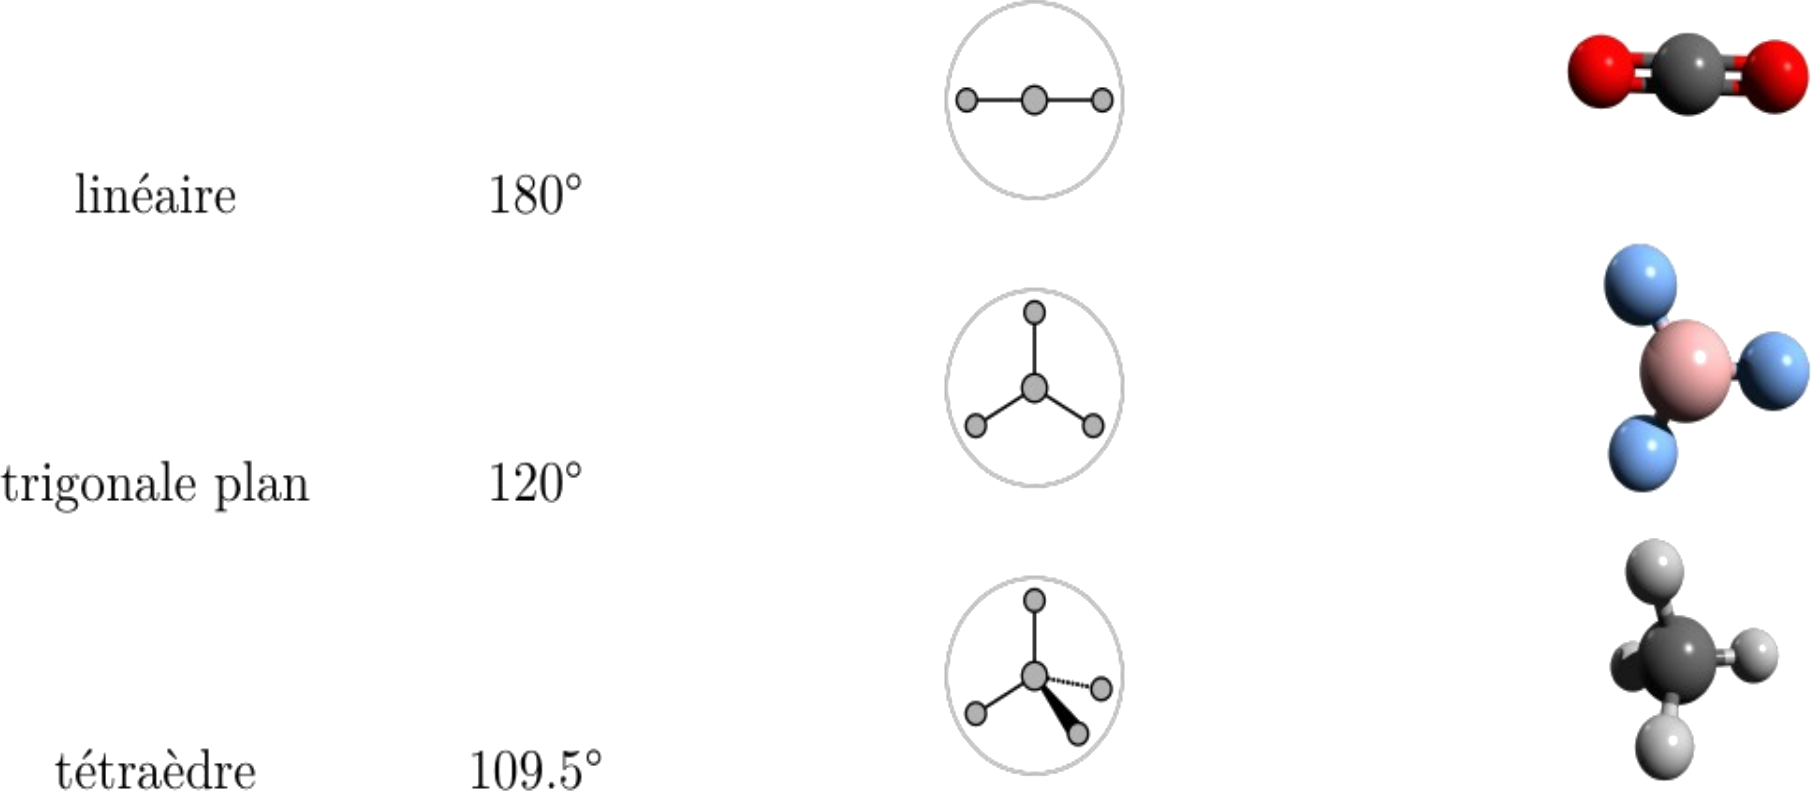
\includegraphics[width=\textwidth]{vsepr.png}
    \caption{Formes à connaître}
    \label{fig:vsepr}
\end{figure}



\subsubsection{Géométrie Linéaire}
La géométrie linéaire se produit lorsque l'atome central est entouré de deux paires
d'électrons liantes et aucune paire libre. Les angles de liaison sont de $180^\circ$.
\begin{itemize}
    \item Exemple~: \ce{CO2} (dans ce cas, ce sont des doubles liaisons qui se repoussent à 180°)
\end{itemize}

\subsubsection{Géométrie Trigonale Plane}
La géométrie trigonale plane se produit lorsque l'atome central est entouré de
trois paires d'électrons liantes et aucune paire libre. Les angles de liaison sont de $120^\circ$.
\begin{itemize}
    \item Exemple~: \ce{BF3}
\end{itemize}

\subsubsection{Géométrie Tétraédrique}
La géométrie tétraédrique se produit lorsque l'atome central est entouré de quatre
paires d'électrons liantes et aucune paire libre. Les angles de liaison sont de $109.5^\circ$.
\begin{itemize}
    \item Exemple~: \ce{CH4}
\end{itemize}

\subsection{Explication des Formes}
Les géométries mentionnées ci-dessus sont déterminées par la disposition des paires
d'électrons autour de l'atome central~:
\begin{itemize}
    \item \textbf{Deux paires d'électrons}~: Les paires se placent à l'opposé l'une de l'autre,
    formant une géométrie linéaire.
    \item \textbf{Trois paires d'électrons}~: Les paires se répartissent dans un plan à
    $120^\circ$ l'une de l'autre, formant une géométrie trigonale plane.
    \item \textbf{Quatre paires d'électrons}~: Les paires se répartissent dans
    l'espace tridimensionnel, formant une géométrie tétraédrique avec des angles de $109.5^\circ$.
\end{itemize}

\subsection{Influence des Paires Libres}
Les paires libres influencent également la géométrie moléculaire~:
\begin{itemize}
    \item Une paire libre sur l'atome central réduit les angles de liaison en raison de la plus
    grande répulsion qu'elle exerce par rapport aux paires liantes.
    \item Par exemple, dans \ce{NH3}, la présence d'une paire libre sur l'azote réduit les angles
    de liaison à environ $107^\circ$, donnant une géométrie pyramidale.
\end{itemize}

\end{document}

